\section{Findings}

\subsection{RQ$_1$: \rqone}
\label{phase1-results}

\textit{Activities} were the most mentioned element in the answers. 35 of the 45 respondents answered its question about good practices, while 38 respondents answered its question about bad practices.
The element that received the least number of responses about good practices was \textit{Listener}, being answered by 10 of the 45 participants. The elements that received the least number of responses about bad practices were \textit{Style} resources and \textit{Drawable}, both of which were answered by only 9 of the 45 participants. 

The coding process resulted in 46 categories. To derive a code smell, we considered 
all the 22 categories that presented occurrences greater than or equal to five, based on the number of Nielsen \cite{NielsenMagicNumber:00}.
Of the 22, we disregarded 2 more because they were (i) a traditional code smell (Large Class) and (ii) one aspect of object orientation (Inheritance). 

\textcolor{red}{if we have space, put back the tab:smells with their summaries}
% Table \ref{tab:Smells} presents the list and a brief description of the 20 proposed Android code smells. The first 9 code smells affect Android presentation layer components, the next 11 affect Android resources.

In the following paragraphs we present in a textual way the definition of code smells, as well as the elements affected by each code smell and related symptoms. 
Definitions were based on the answers obtained. 
The number in parenthesis shows the number of times that smell appeared in the answers.
In the appendix, we show the the entire coding results~\ref{appendix:smells-purpose-of-solution}.


\noindent
\textsc{\textbf{{\small Brain UI Component}}}$^{(60)}$: \textit{Activities}, \textit{Fragments}, \textit{Adapters}, and \textit{Listeners} should contain only code responsible for presenting, interacting and updating the UI. The existence of code related to business logic, IO operations, conversion of data or static fields in these elements are signs of code smell.


\noindent
\textbf{\textsc{{\small Obscure names}}}$^{(24)}$:
The smell happens when resources (\textit{layout}, \textit{string}, \textit{style}, \textit{drawables}) do not follow a naming pattern. This may happen in the file name as well as in the names used internally in the resource. 


\noindent
\textbf{\textsc{{\small Magic Resource}}}$^{(23)}$:
The smell happens when resources are hard-coded instead of pointing
to an existing resource.


\noindent
\textbf{\textsc{{\small Deep Nested Layout}}}$^{(19)}$:
Deep nesting when constructing \textit{layout} resources is considered 
a code smell. Interestingly, the official Android website has more
information and even provides automated tools to deal with such
problem~\cite{OptmizingViewHierarchies}.

\noindent
\textbf{\textsc{{\small Unnecessary Image}}}$^{(18)}$:
Android has several resources that can replace some images. The smell
emerges when the system has images with, for example, 
pure solid colors or gradients, that could be replaced by
Android's native \textit{shapes}.

\noindent
\textbf{\textsc{{\small Coupled UI Component}}}$^{(18)}$: \textit{Fragments}, \textit{Adapters}, and \textit{Listeners}, so that they can be reused, they should not have direct reference to who uses them. The existence of direct reference to \textit{Activities} or \textit{Fragments} in these elements is an evidence of code smell.

\noindent
\textsc{\textbf{{\small Suspicious Behavior}}}$^{(17)}$: \textit{Activities}, \textit{Fragments}, and \textit{Adapters} should not be responsible for implementing event behavior. The use of anonymous classes, internal classes, or polymorphism (via implements) to implement \textit{Listeners} to respond to user events is a sign of code smell.
 

\noindent
\textbf{\textsc{{\small Long or Repeated Layout}}}$^{(14)}$:
The code smell emerges when 
long or duplicated \textit{layout} resources (instead of good reuse) 
happen in the source code.


\noindent
\textsc{\textbf{{\small Fool Adapter}}}$^{(13)}$: 
It happens when \textit{Adapters} do not reuse instances of the \textit{views} that
represent the fields that will be populated for each item of a collection by means
of the \textit{View Holder} pattern. 

\noindent
\textbf{\textsc{{\small Missing Image}}}$^{(12)}$:
The code smell happens when the system contains only a single
version of its .png, .jpg, or .gif images. The Android platform
requires images to be available in more than one size or resolution
to perform optimizations.


\noindent
\textsc{\textbf{{\small Excessive Use of Fragments}}}$^{(9)}$: 
The smell emerges when \textit{Fragments} are used in an application
that does not (need to) support tablets. It also happens when \textit{Fragments} are
used in only a single screen of the app.

\noindent
\textsc{\textbf{{\small UI Component Doing I/O}}}$^{(9)}$:
It happens when \textit{Activities}, \textit{Fragments} and \textit{Adapters} perform
I/O operations, such as database and file access.


\noindent
\textsc{\textbf{{\small No Use of Fragments}}}$^{(8)}$: 
The code smell emerges when view components such as 
\textit{EditTexts}, \textit{Spinners}, are directly used by an \textit{Activity};
in such cases, a \textit{Fragment} should be introduced.


\noindent
\textbf{\textsc{{\small God Style Resource}}}$^{(8)}$:
Long \textit{style} resources. Symptoms of this smell happen when
all styles are defined in the same \textit{styles.xml}.

\noindent
\textbf{\textsc{{\small God String Resource}}}$^{(8)}$:
Long \textit{string} resources. Developers should separate their string
resources according to some rule, e.g., one string resource per screen.

\noindent
\textbf{\textsc{{\small Duplicate Style Attributes}}}$^{(7)}$:
The existence of duplicated style attributes in \textit{layout} or
\textit{style} resources, when they could be reused, is an indication
of this code smell.

\noindent
\textsc{\textbf{{\small Flex Adapter}}}$^{(6)}$ \textit{Adapters} 
should be responsible for populating a \textit{view} from a single object.
The code smell emerges when \textit{Adapters} contain
business logic and takes business decisions. 


\noindent
\textsc{\textbf{{\small Absence of an Architecture}}}$^{(6)}$: 
The smell emerges when one can not easily identify how the components
are organized. Developers can not identify whether the application
makes use of Model View Controller (MVC), Model View Presenter (MVP),
or Model View ViewModel (MVVM).


\noindent
\textbf{\textsc{{\small Inappropriate String Reuse}}}$^{(6)}$:
The smell happens when developers reuse the same \textit{string} in different
parts of the system, just because the string is coincidentally the same.


\noindent
\textbf{\textsc{{\small Hidden Listener}}}$^{(5)}$:
\textit{Layout} resources should only be responsible for presenting data.
It is a smell when these resources also configure the listener that
will respond to its events, such as \textit{onClick}. Such decision
makes it harder for developers to identify which listeners are being used.

\subsection{RQ$_2$: \rqtwo}
\label{phase2-results}

% Participaram desta etapa da pesquisa 201 desenvolvedores de 3 continentes e 14 países diferentes. Brasileiros representam 78\%, e vieram de 18 estados diferentes. Deste modo, apesar da abrangência geográfica, entendemos que os resultados expressam majoritariamente a percepção de desenvolvedores brasileiros. 15\% dos participantes possuem uma ou mais pós-graduações e 61\% são graduados. 57\% possuem de 20 a 35 anos.

Nossos resultados mostraram que os 20 maus cheiros propostos são considerados, em diferentes níveis, importantes e se apresentam com diferentes frequências no dia a dia do desenvolvimento Android. As distribuições relativas de frequência e importância, sobre cada afirmação apresentada no questionário, pode ser conferida nos Apêndices \ref{appendix-phase2-frequence-table} (afirmações de frequência) e \ref{appendix-phase2-importance-table} (afirmações de importância).

% Para os maus cheiros que foram apresentadas no questionário mais de uma afirmação de importância ou frequência, se mostraram com distribuição relativa muito semelhantes, variando de 6\% a no máximo 10\% de uma afirmação a outra.

\subsubsection{Resultados Gerais}
\label{phase2-general-results}

Para análise dos maus cheiros extraímos dados estatísticos de moda (MO), mediana (ME) e desvio padrão (DP) de importância e frequência para cada um dos maus cheiros propostos. Utilizamos a MO como um classificador do mau cheiro, ou seja, se ele recebeu majoritariamente a resposta ``importante'', o classificamos como importante. Estes dados são apresentados na Tabela \ref{tab:SmellFrequencyImportance} onde podemos observar que todos os maus cheiros apresentam MO de importância maior ou igual a 3, ou seja, de ``razoavelmente importante'' a ``muito importante''. Em contrapartida, com relação à frequência, três maus cheiros (\textsc{\small Fool Adapter}, \textsc{\small Hided Listener} e \textsc{\small No Fragment Usage}) apresentaram MO igual a 2, ``raramente'', todos os demais apresentaram MO maior ou igual a 3, ou seja, de ``às vezes'' até ``muito frequente''.

\begin{table}[!htb]
\centering
\renewcommand*{\arraystretch}{1}
\footnotesize
\caption{Mediana (ME), moda (MO) e desvio padrão (DP) sobre a percepção da importância dos maus cheiros relacionados a componentes da camada de apresentação Android.}
\begin{tabular}{@{}p{5cm}cccp{.5cm}ccc@{}}
\toprule
\multirow{2}{*}{\textbf{Mau Cheiro}} & \multicolumn{3}{c}{\textbf{Importância}} & & \multicolumn{3}{c}{\textbf{Frequência}} \\ \cmidrule{2-4} \cmidrule{6-8}
                                      & \textbf{ME} & \textbf{MO} & \textbf{DP} & & \textbf{ME} & \textbf{MO} & \textbf{DP} \\
\bottomrule
\textsc{Brain UI Component} & 5 & 5 & 1,05 & & 3 & 4 & 1,19 \\
\textsc{Magic Resource} & 4 & 5 & 1,00 & & 3 & 4 & 1,24 \\
\textsc{Avoid Tradicional Images} & 4 & 5 & 0,95 & & 3 & 4 & 1,23 \\
\textsc{Layout Long or Repeated} & 4 & 5 & 0,95 & & 4 & 4 & 1,07 \\
\textsc{Missing Image} & 5 & 5 & 0,95 & & 3 & 4 & 1,25 \\
\textsc{Coupled UI Component} & 4 & 5 & 1,02 & & 3 & 3 & 1,15 \\
\textsc{Classes de UI Fazendo IO} & 5 & 5 & 1,03 & & 3 & 3 & 1,29 \\
% \textsc{Componente de UI Zumbi} & 5 & 5 & 0,88 & & 3 & 3 & 1,16 \\
\textsc{Absence of Architecture} & 5 & 5 & 0,82 & & 3 & 3 & 1,30 \\
\textsc{Flex Adapter} & 4 & 5 & 0,91 & & 3 & 3 & 1,15 \\
\textsc{Resource Name Non Patterned} & 5 & 5 & 0,88 & & 3 & 3 & 1,24 \\
\textsc{Fool Adapter} & 5 & 5 & 0,93 & & 2 & 2 & 1,20 \\
\textsc{Hided Listener} & 4 & 5 & 1,23 & & 2 & 2 & 1,29 \\
\textsc{God Style Resource} & 4 & 4 & 1,06 & & 4 & 5 & 1,18 \\
\textsc{Messy String Resource} & 3 & 4 & 1,22 & & 4 & 5 & 1,18 \\
\textsc{Suspicious Behavior} & 3 & 4 & 1,19 & & 3 & 4 & 1,19 \\
\textsc{Deep Nested Layout} & 4 & 4 & 1,12 & & 4 & 4 & 1,06 \\
\textsc{Repeated Style Attributes} & 4 & 4 & 0,86 & & 4 & 4 & 1,11 \\
\textsc{No Fragment Usage} & 3 & 4 & 1,34 & & 3 & 2 & 1,21 \\
\textsc{Inappropriate String Reuse} & 3 & 3 & 1,29 & & 4 & 4 & 1,12 \\
\textsc{Uso Excessivo de Fragment} & 3 & 3 & 1,36 & & 3 & 3 & 1,17 \\
\toprule
DP Médio &  &  & 1.05 &  & &  & 1.19 \\
% \toprule
% \multicolumn{8}{@{}l@{}}{DP = Desvio Padrão, MO = Moda, ME = Média.} \\
\bottomrule
\end{tabular}
\label{tab:SmellFrequencyImportance}
\end{table}


Entendemos este resultado de forma positiva pois, apesar de alguns sintomas não serem tão frequentes, ainda assim são considerados com algum nível de importância de se mitigar, reforçando também a relevância desta pesquisa pois damos os primeiros passos no sentido da automatização da identificação desses maus cheiros. Com base no DP, podemos observar que, de modo geral, existe uma concordância maior sobre a importância dos maus cheiros do que sobre a frequência, pois a média do DP de importância é de 1,05, ligeiramente menor que a média do DP de frequência, que é de 1,19.

Quanto menor o DP maior a concordância entre os participantes sobre determinado mau cheiro. Podemos observar que os maus cheiros que tiveram maior concordância com relação à sua importância foram: \textsc{\small Flex Adapter}, \textsc{\small Fool Adapter}, \textsc{\small Repeated Style Attributes}, \textsc{\small Absence of Architecture}, \textsc{\small Missing Image}, \textsc{\small Avoid Tradicional Images}, \textsc{\small Layout Long or Repeated}, \textsc{\small Resource Name Non Patterned}, todos com DP menor que 1. Sobre a concordância relacionada à frequência, nenhum dos maus cheiros obteve DP menor que 1, mas os mais próximos, indicando maior concordância sobre sua frequência são: \textsc{\small Deep Nested Layout} com DP de 1,06 e \textsc{\small God Style Resource} com DP 1,07.


\subsubsection{Importância dos Maus Cheiros}

Para análise dos dados, simplificamos a escala \textit{likert} de importância de modo que, os maus cheiros de MO 3, ``razoavelmente importante'', são classificados como sendo de \textbf{\small importância moderada}, os maus cheiros de MO 4 ou 5, respectivamente ``importante'' e ``muito importante'', são classificados de \textbf{\small importância alta}. Nenhum mau cheiro teve MO 1 ou 2, respectivamente ``não é importante'' e ``pouco importante'', logo, não criamos classificações para essas opções.

A Tabela \ref{tab:SmellImportance} apresenta a lista dos maus cheiros de acordo com seu nível de importância, alta ou moderada. Podemos observar que as duas primeiras colunas contém os 18 maus cheiros classificados com \textbf{\small importância alta}. Dentre eles, a maioria dos maus cheiros (10) afetam recursos Android: \textsc{\small God Style Resource}, \textsc{\small Deep Nested Layout}, \textsc{\small Repeated Style Attributes}, \textsc{\small Resource Name Non Patterned}, \textsc{\small Magic Resource}, \textsc{\small Missing Image}, \textsc{\small Avoid Tradicional Images}, \textsc{\small Layout Long or Repeated}, \textsc{\small Messy String Resource} e \textsc{\small Hided Listener}.

\begin{table}[!htb]
\centering
\renewcommand*{\arraystretch}{1}
\footnotesize
\caption{Listagem dos maus cheiros da camada de apresentação Android de acordo com seu nível de importância, alta ou moderada.}
\begin{tabular}{@{}p{5.2cm}p{5.2cm}p{5.2cm}@{}}
\toprule
\multicolumn{2}{c}{\textbf{Importância Alta}} & \multicolumn{1}{c}{\textbf{Importância Moderada}}  \\
\bottomrule
\textsc{\scriptsize Flex Adapter}              & \textsc{\scriptsize Repeated Style Attributes} & \textsc{\scriptsize Inappropriate String Reuse} \\
\textsc{\scriptsize Fool Adapter}            & \textsc{\scriptsize Suspicious Behavior}        & \textsc{\scriptsize Uso Excessivo de Fragment} \\
\textsc{\scriptsize Absence of Architecture}       & \textsc{\scriptsize Deep Nested Layout} \\
\textsc{\scriptsize Classes de UI Fazendo IO}      & \textsc{\scriptsize God Style Resource}       \\
\textsc{\scriptsize Coupled UI Component}     & \textsc{\scriptsize No Fragment Usage}           \\
\textsc{\scriptsize Brain UI Component}      & \textsc{\scriptsize Messy String Resource}   \\
\textsc{\scriptsize Magic Resource}                & \textsc{\scriptsize Missing Image}               \\
\textsc{\scriptsize Avoid Tradicional Images}& \textsc{\scriptsize Layout Long or Repeated}      \\
\textsc{\scriptsize Hided Listener}            & \textsc{\scriptsize Resource Name Non Patterned}\\
\toprule
\multicolumn{2}{c}{18} & \multicolumn{1}{c}{2}  \\
\bottomrule
\end{tabular}
\label{tab:SmellImportance}
\end{table}

Enquanto que 8 dos maus cheiros de \textbf{\small importância alta} afetam componentes da camada de apresentação Android: \textsc{\small Flex Adapter}, \textsc{\small Fool Adapter}, \textsc{\small Absence of Architecture}, \textsc{\small Classes de UI Fazendo IO}, \textsc{\small Brain UI Component}, \textsc{\small Repeated Style Attributes}, \textsc{\small Suspicious Behavior} e \textsc{\small No Fragment Usage}. Apenas 2 maus cheiros: \textsc{\small Inappropriate String Reuse} e \textsc{\small Uso Excessivo de Fragment}, listados na última coluna da tabela, são de \textbf{\small importância moderada}, sendo 1 relacionado a recursos e outro componentes da camada de apresentação Android.

A Figura \ref{fig:phase2-results-importance} apresenta a distribuição relativa de importância dos maus cheiros. Apresentamos negativo (em vermelho) o percentual relacionado às respostas ``não é importante''.

\begin{figure}
  \centering
  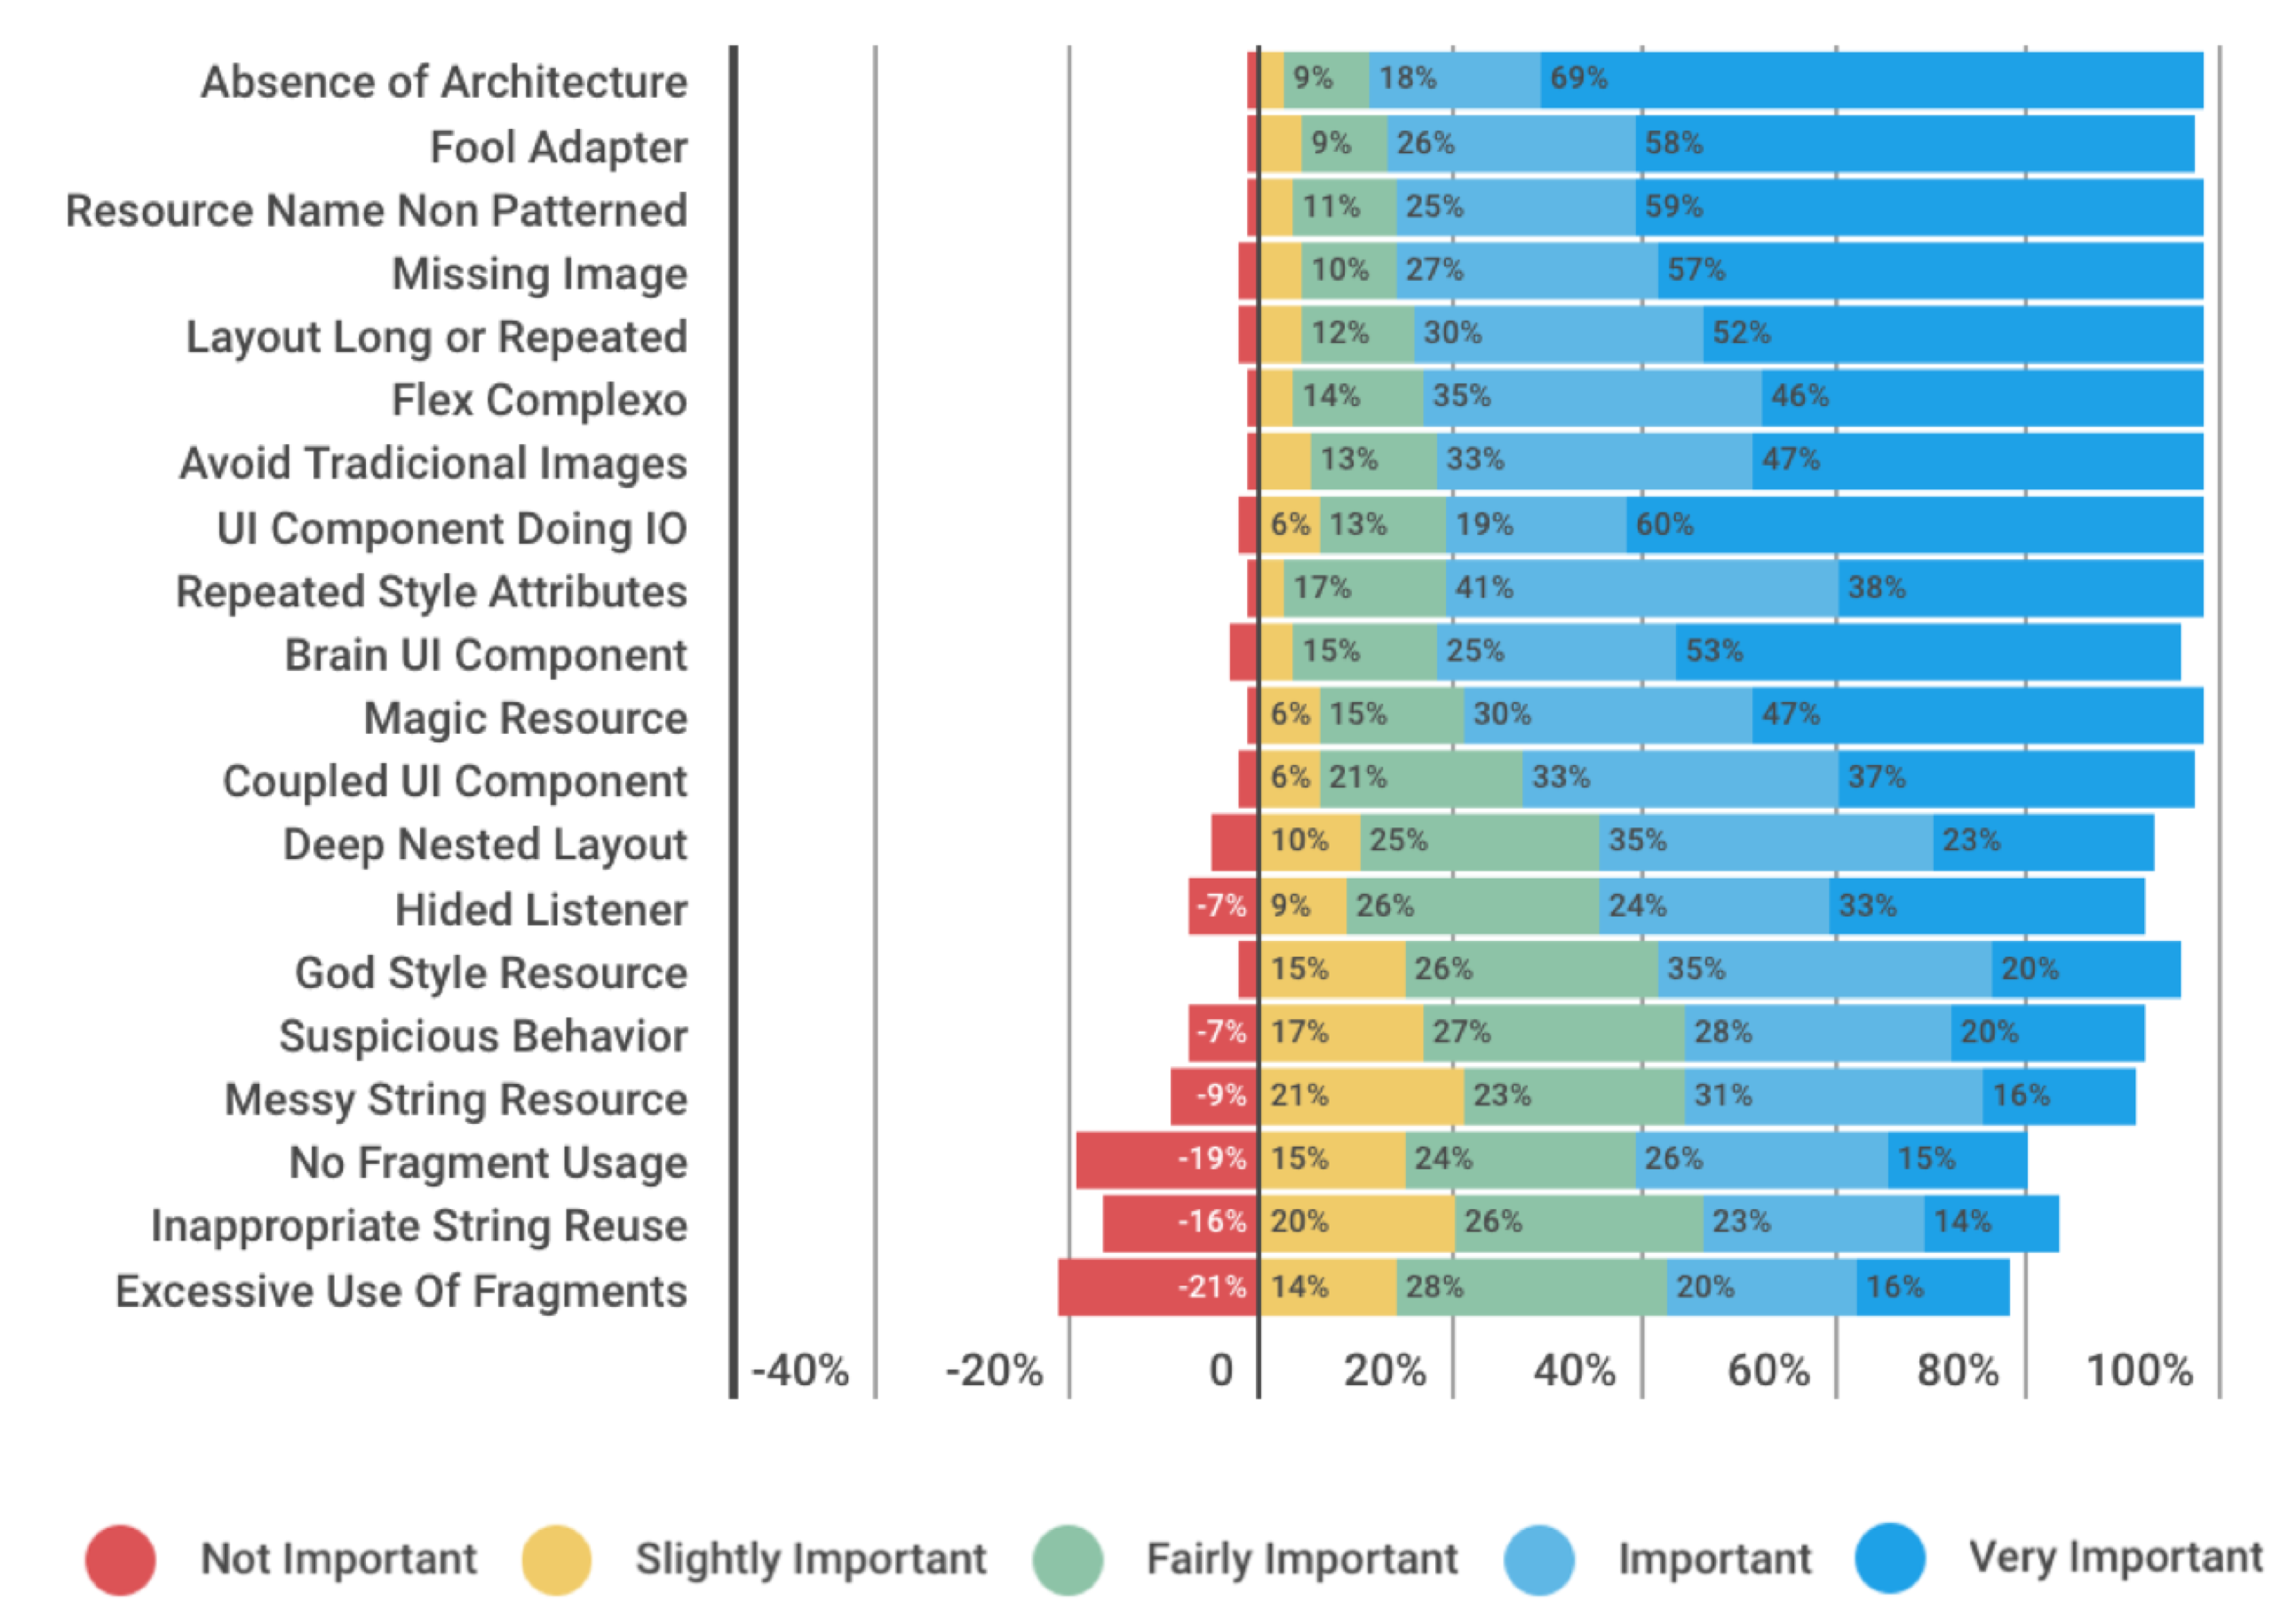
\includegraphics[width=1\columnwidth]{phase2-results-importance3-en.png}
  \caption{Distribuição relativa de importância dos maus cheiros propostos.}
  \label{fig:phase2-results-importance}
  % \vspace{-.5cm}
\end{figure}

Os três maus cheiros considerados menos importantes foram \textsc{\small Inappropriate String Reuse}, \textsc{\small No Fragment Usage} e \textsc{\small Uso Excessivo de Fragment}, com mais de 16\% dos participantes indicando ``não é importante'', menos de 26\% indicando ``importante'' e menos de 16\% indicando ``muito importante''. São os mesmos que tiveram menor concordância com relação à sua importância, todos com DP acima de 1,28. Esses dados sugerem que desenvolvedores Android ainda têm dúvidas sobre o impacto negativo desses maus cheiros no código.


\subsubsection{Frequência dos Maus Cheiros}

Para análise dos dados, simplificamos a escala \textit{likert} de frequência de modo similar ao de importância, onde maus cheiros de MO 2, ``raramente'', são classificados como \textbf{\small frequência baixa}, os maus cheiros de MO 3, ``às vezes'', são classificados como \textbf{\small frequência moderada} e os maus cheiros de MO 4 ou 5, respectivamente ``frequente'' e ``muito frequente'', são classificados de \textbf{\small frequência alta}. Nenhum mau cheiro teve MO 1, ``nunca'', e portanto não criamos classificação para essa opção. A Tabela \ref{tab:SmellFrequency} apresenta a lista dos maus cheiros de acordo com seu nível de frequência, alta, moderada ou baixa.

\begin{table}[!htb]
\centering
\renewcommand*{\arraystretch}{1}
\footnotesize
\caption{Listagem dos maus cheiros da camada de apresentação Android de acordo com seu nível de frequência, alta, moderada ou baixa.}
\begin{tabular}{@{}p{5.2cm}p{5.2cm}p{5.2cm}@{}}
\toprule
\multicolumn{1}{c}{\textbf{Frequência Alta}} & \multicolumn{1}{c}{\textbf{Frequência Moderada}} & \multicolumn{1}{c}{\textbf{Frequência Baixa}} \\
\bottomrule
\textsc{\scriptsize Repeated Style Attributes}  & \textsc{\scriptsize Flex Adapter}               & \textsc{\scriptsize Fool Adapter} \\
\textsc{\scriptsize Brain UI Component}       & \textsc{\scriptsize Absence of Architecture}        & \textsc{\scriptsize Hided Listener} \\
\textsc{\scriptsize Missing Image}                & \textsc{\scriptsize Classes de UI Fazendo IO}       & \textsc{\scriptsize No Fragment Usage} \\
\textsc{\scriptsize Avoid Tradicional Images} & \textsc{\scriptsize Coupled UI Component}      \\
\textsc{\scriptsize Layout Long or Repeated}       & \textsc{\scriptsize Uso Excessivo de Fragment}      \\
\textsc{\scriptsize Deep Nested Layout}  & \textsc{\scriptsize Suspicious Behavior}         \\
\textsc{\scriptsize God Style Resource}        & \textsc{\scriptsize Resource Name Non Patterned} \\
\textsc{\scriptsize Magic Resource}                 \\
\textsc{\scriptsize Inappropriate String Reuse}     \\
\textsc{\scriptsize Messy String Resource}    \\
\toprule
\multicolumn{1}{c}{10} & \multicolumn{1}{c}{7} & \multicolumn{1}{c}{3}\\
\bottomrule
\end{tabular}
\label{tab:SmellFrequency}
\end{table}

É interessante notar que, maus cheiros em recursos são percebidos mais frequentemente que os maus cheiros em componentes da camada de apresentação Android. Podemos observar na Tabela \ref{tab:SmellFrequency} que, 9 dentre os 10 maus cheiros de \textbf{\small frequência alta} são em recursos Android: \textsc{\small Repeated Style Attributes}, \textsc{\small Missing Image}, \textsc{\small Avoid Tradicional Images}, \textsc{\small Layout Long or Repeated}, \textsc{\small Deep Nested Layout}, \textsc{\small God Style Resource}, \textsc{\small Magic Resource}, \textsc{\small Inappropriate String Reuse} e \textsc{\small Messy String Resource}. Enquanto que apenas o mau cheiro de \textbf{\small frequência alta}, \textsc{\small Brain UI Component}, é relacionado a componentes da camada de apresentação Android.

Nos demais níveis de frequência, essa situação se inverte, sendo os maus cheiros em componentes da camada de apresentação Android, maioria. Dentre os maus cheiros de \textbf{\small frequência moderada}, 6 dentre os 7 são relacionados a componentes: \textsc{\small Flex Adapter}, \textsc{\small Absence of Architecture}, \textsc{\small Classes de UI Fazendo IO}, \textsc{\small Coupled UI Component}, \textsc{\small Uso Excessivo de Fragment} e \textsc{\small Suspicious Behavior}. Apenas o mau cheiro \textsc{\small Resource Name Non Patterned} é relacionado a recursos Android. Dentre os maus cheiro de \textbf{\small frequência baixa}, 2 dentre os 3 são relacionados a componentes da camada de apresentação Android: \textsc{\small Fool Adapter} e \textsc{\small No Fragment Usage}. E apenas o mau cheiro \textsc{\small Hided Listener} é relacionado a recursos Android.

\begin{figure}
  \centering
  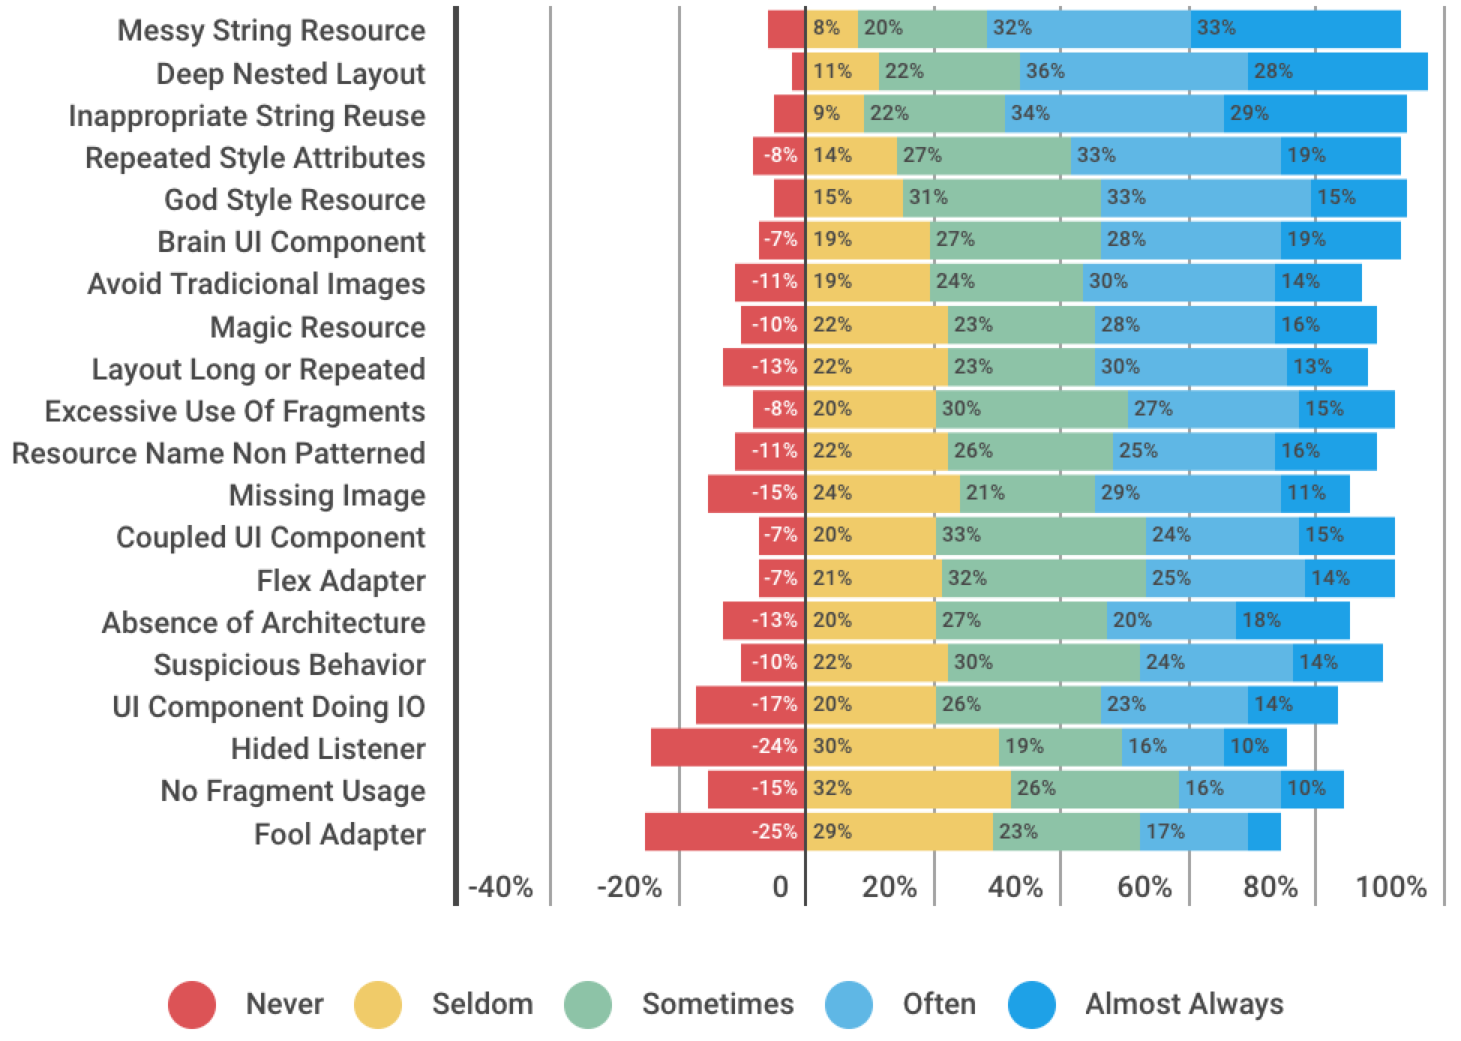
\includegraphics[width=1\columnwidth]{phase2-results-frequence-en.png}
  \caption{Distribuição relativa de frequência dos maus cheiros propostos.}
  \label{fig:phase2-survey-frequence}
  % \vspace{-.5cm}
\end{figure}

A Figura \ref{fig:phase2-survey-frequence} apresenta a distribuição relativa de frequência dos maus cheiros. Apresentamos negativo (em vermelho) o percentual relacionado às respostas ``nunca''. Os maus cheiros menos percebidos (com mais de 20\% de respostas ``nunca'') foram \textsc{\small Fool Adapter} (25\%) e \textsc{\small Hided Listener} (24\%). Todos os demais maus cheiros são percebidos no dia a dia, com frequência moderada ou alta, por pelo menos 75\% dos participantes.

\textsc{\small Fool Adapter} foi o mau cheiro menos percebido no dia a dia por desenvolvedores Android (25\% dos participantes indicaram ``nunca''). Entretanto ele é o segundo considerado mais importante (58\% dos participantes indicaram ``muito importante'' e 26\% indicaram ``importante''). Esses dados sugerem que desenvolvedores já estão cientes dos benefícios do uso do padrão \textit{ViewHolder} \cite{AluraViewHolder} e encontraram formas de mitigar este mau cheiro. Na seção \ref{sec:discussoes} realizamos uma breve discussão sobre esse resultado.

\textsc{\small Hided Listener} foi o segundo mau cheiro menos percebido no dia a dia por desenvolvedores Android (24\% dos participantes indicaram ``nunca''). Entretanto se apresenta dentre os maus cheiros considerados mais importantes (33\% dos participantes indicaram ``muito importante'' e 24\% indicaram ``importante''). Esses dados sugerem que os desenvolvedores consideram importante evitar o uso do atributo \textit{onClick} em XMLs de \textit{layout} e aparentemente, muitos desenvolvedores já estão cientes disso no dia a dia, uma vez que ele se apresenta dentre os 6 menos percebidos. \\


\begin{square}
  \small
  Nossos resultados mostram que os maus cheiros propostos são considerados importantes e frequentes no dia a dia do desenvolvimento Android (QP$_2$).
\end{square}




% -*- root: dissertation.tex -*-
\subsection{QP$_3$ Percepção dos Desenvolvedores sobre os Maus Cheiros Android}
\label{phase3-results}

Nossos resultados mostram que códigos afetados por 6 dos 7 maus cheiros avaliados são percebidos como códigos problemáticos por desenvolvedores Android, são eles: \textsc{\small Brain UI Component}, \textsc{\small Coupled UI Component}, \textsc{\small Suspicious Behavior}, \textsc{\small Flex Adapter}, \textsc{\small Deep Nested Layout} e \textsc{\small Repeated Style Attributes}. Não foi possível concluir a percepção sobre o mau cheiro \textsc{\small God Style Resource} pois a média de 30 pontos não foi suficiente para chegarmos a uma conclusão, sendo necessário coletar mais dados. A seguir apresentamos detalhes das percepções dos desenvolvedores sobre os maus cheiros avaliados.

% Com o objetivo de aumentar a confiabilidade do experimento, nosso objetivo foi obter em média 30 pontos de observação para cada mau cheiro avaliado. Para 6 maus cheiros essa quantidade de pontos foi suficiente, porém para o mau cheiro \textsc{\small God Style Resource} não,


\subsubsection{Resultados}
\label{sec:results-phase3}

Na Figura \ref{fig:components-violins}, apresentamos os gráficos violino que consolidam a percepção de desenvolvedores sobre os 4 maus cheiros relacionados a componentes da camada de apresentação Android (\textsc{\small Brain UI Component}, \textsc{\small Coupled UI Component}, \textsc{\small Suspicious Behavior} e \textsc{\small Flex Adapter}) contra componentes Android limpos. De modo similar, na Figura \ref{fig:resources-violins}, apresentamos os gráficos violino que consolidam a percepção de desenvolvedores sobre os 3 maus cheiros relacionados à recursos Android (\textsc{\small Deep Nested Layout}, \textsc{\small Repeated Style Attributes} e \textsc{\small God Style Resource}) contra recursos limpos.

\begin{figure*}[!htb]
\centering
\imagewidth=0.54\textwidth
\captionsetup[subfigure]{width=.9\imagewidth,justification=raggedright}%
\begin{subfigure}[t]{.49\textwidth}
  \centering
  \hspace*{-1cm}%
  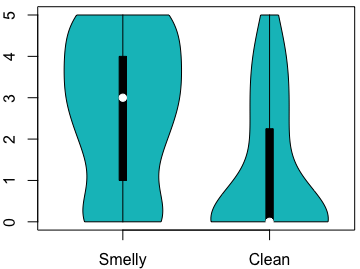
\includegraphics[width=.8\textwidth]{phase3-components-clean-smelly-violins-cutted-en.png}
  \caption{Components.}
  \label{fig:components-violins}
\end{subfigure}
\begin{subfigure}[t]{.49\textwidth}
  \centering
  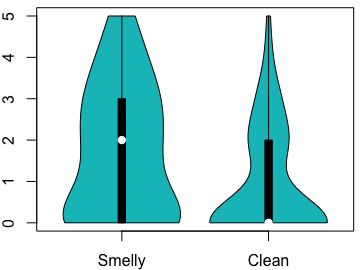
\includegraphics[width=.8\textwidth]{phase3-resources-clean-smelly-violins-cutted-en.png}
  \caption{Resources.}
  \label{fig:resources-violins}
\end{subfigure}%
\caption{Analysis of severity in components and resourcecs smelly and clean.}
\label{fig:smelly-clean-consolidado}
% \vspace{-.5cm}
\end{figure*}

No eixo y, 0 (zero) indica os códigos não percebidos pelos desenvolvedores como problemáticos (ou seja, responderam ``não'' à questão: ``\emph{Esta classe exibe algum problema de design e/ou implementação?}''), enquanto que os valores de 1 a 5 indicam o nível de severidade para o problema percebido pelo desenvolvedor. No eixo x, os gráficos são autoexplicativos. Nos parágrafos seguintes explicamos os dados de cada gráfico de modo que, as medianas são indicadas pela bolinha branca e o 3º quartil (Q3) é representado pela linha preta mais grossa na vertical.

Podemos observar na Figura \ref{fig:components-violins} que componentes afetados pelos maus cheiros Android tiveram mediana de severidade igual a 3 (Q3 = 4). Isso indica que, como esperado, desenvolvedores percebem códigos afetados pelos maus cheiros em componentes da camada de apresentação Android como problemáticos. Como comparação, componentes Android limpos tiveram mediana de severidade igual a 0 (Q3 = 2). A diferença na percepção dos desenvolvedores entre componentes Android mau cheirosos e componentes limpos é estatisticamente significante ($\alpha$ = 1,18e-06) com médio tamanho de efeito (\textit{d} = 0,46).

Na Figura \ref{fig:resources-violins}, podemos observar que recursos afetados pelos maus cheiros Android tiveram mediana de severidade é igual a 2 (Q3 = 3). Isso mostra que, recursos afetados pelos maus cheiros Android são percebidos como problemáticos, ainda que menos que os maus cheiros em componentes Android. Como comparação, recursos Android limpos tiveram mediana de severidade igual a 0 (Q3 = 2). A diferença na percepção dos desenvolvedores entre os recursos mau cheirosos e recursos limpos também é estatisticamente significante ($\alpha$ = 1,24e-03) com pequeno tamanho de efeito (\textit{d} = 0,29).

 % - bem como de componentes e recursos de \textit{Style} e \textit{Layout} limpos - Figura \ref{fig:clean-violins}.
Além disso, relatamos a percepção dos desenvolvedores sobre cada mau cheiro Android individualmente na Figura \ref{fig:smellys-violins}. O mau cheiro \textsc{\small Coupled UI Component} (CA) é o mais percebido pelos desenvolvedores e com maior gravidade, apresenta mediana de severidade igual a 4 (Q3 = 5). Em seguida temos os maus cheiros \textsc{\small Brain UI Component} (CC), \textsc{\small Flex Adapter} (AC) e \textsc{\small Suspicious Behavior} (CS) todos com mediana de severidade igual a 3. Isso indica que, como esperado, são percebidos pelos desenvolvedores como sendo seriamente problemáticos. Podemos notar que, de modo geral, recursos afetados pelos maus cheiros Android -- \textsc{\small God Style Resource} (LE), \textsc{\small Deep Nested Layout} (LA) e \textsc{\small Repeated Style Attributes} (AR) -- foram percebidos com menor severidade, mediana 1 e 2, do que componentes afetados pelos maus cheiros, todos com mediana de severidade maior ou igual a 3 (Q3 $\geq$ 3).  \\


\begin{figure*}[!htb]
\centering
\imagewidth=0.54\textwidth
\captionsetup[subfigure]{width=.9\imagewidth,justification=raggedright}%
\begin{subfigure}[t]{.48\textwidth}\centering
  \hspace*{-1cm}%
  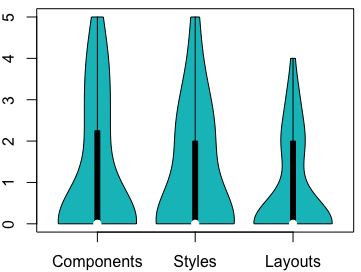
\includegraphics[width=.82\textwidth]{phase3-clean-violins-cutted-en.png}
  \caption{Components=\textit{Activities}, \textit{Fragments}, \textit{Adapters} or \textit{Listeners} cleans. Styles=Clean \textit{style} resources. Layout= Clean \textit{layout} resources.}
  % \hspace*{-1cm}%
  \label{fig:clean-violins}
\end{subfigure}
\begin{subfigure}[t]{.48\textwidth}\centering
  % \hspace*{-1cm}%
  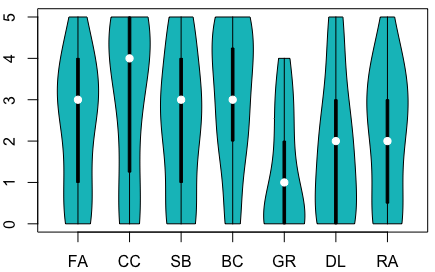
\includegraphics[width=1\textwidth]{phase3-smellys-violins2-cutted-en.png}
  \caption{FA=Flex Adapter, CC=Coupled UI Component, SB=Suspicious Behavior, BC=Brain UI Component, GR=God Style Resource, DL=Deep Nested Layout
, AR=Repeated Style Attributes.}
  % \hspace*{-1cm}%
  \label{fig:smellys-violins}
\end{subfigure}%
\caption{Analysis of severity of clean codes segmented by groups and codes affected by code smells evaluated.}
\label{fig:}
% \vspace{-.5cm}
\end{figure*}

A Figura \ref{fig:clean-violins} apresenta os gráficos violino sobre a percepção dos 3 grupos de códigos limpos: componentes Android, recursos de \textit{style} e recursos de \textit{layout}. Podemos observar que os 3 grupos de códigos apresentam mediana de severidade 0. Isso mostra que, como esperado, os códigos limpos, no geral, foram percebidos como limpos pelos desenvolvedores.

Muitos desenvolvedores, sem conhecer nosso catálogo de maus cheiros Android, foram capazes de identificar corretamente o mau cheiro, dando uma descrição do problema percebido muito próxima a definição do mau cheiro. Por exemplo, um deles ao se deparar com um \textsc{\small Flex Adapter} relatou: \textit{``O método getView é muito longo, com muitos ifs. Dificultando testes, debug e entendimento. me parece que muitas variações de tela podem ser desenhadas nesse método.''}. Outro participante disse simplesmente: \textit{``getView faz muitas coisas. Isso é perigoso para manter.''}.

Também o mau cheiro \textsc{\small God Style Resource}, foi corretamente identificado. Por exemplo, um dos participantes relatou: \textit{``Os temas e estilos poderiam ser separados em arquivos diferentes como por exemplo styles\_dialog.xml, styles\_text\_view.xml, etc inclusive em diretórios de recursos de acordo com nível de API do Android. Também poderia usar herança.''}. Outro participante disse apenas: \textit{``Muitos estilos no mesmo arquivo.''}.

Outro participante ao se deparar com \textsc{\small Coupled UI Component}, relatou: \textit{``Adapter está acoplado a MainActivity, uma vez que a recebe no construtor. O ideal seria abstrair quem está usando o Adapter para que ele possa ser usado por outras activities ou fragments.''}. Outros dois disseram simplesmente: \textit{``Cast direto à MainActivity.''} e \textit{``O DrawerAdapter está acoplado com a MainActivity.''}. Sobre o mau cheiro \textsc{\small Repeated Style Attributes}, um participante relatou: \textit{``1. Muitas dimensões repetidas que tem o mesmo propósito. Elas deveriam estar num lugar centralizado e nomeadas para facilidade de manutenção. 2. Mesma definição de estilo para várias text views. Deveria ser extraídas para styles para melhor manutenção...''}. Outro participante disse: \textit{``Muitos textViews com a mesma estilização, mas não se utiliza um arquivo de de styles para auxiliar.''}.

\begin{table}[!htb]
\centering
\renewcommand*{\arraystretch}{1}
\footnotesize
\caption{Dados estatísticos sobre a percepção negativa por desenvolvedores sobre os maus cheiros avaliados no experimento de código (S$_3$).}
\begin{tabular}{@{}p{7cm}clcc@{}}
\toprule
\textbf{Mau Cheiro} & \multicolumn{1}{c}{\textbf{Valor de p ($\alpha$)}} & \multicolumn{1}{c}{\textbf{Delta de Cliff (\textit{d})}} & \textbf{Mediana} & \textbf{Q3} \\
\toprule
\textsc{\small Coupled UI Component}       &  1,13e-04  &    0,52 (grande) & 4,00         & 5,00 \\
\textsc{\small Suspicious Behavior}          &  1,37e-03  &    0,38 (médio)  & 3,00         & 4,00 \\
\textsc{\small Brain UI Component}        &  4,58e-06  &    0,55 (grande) & 3,00         & 4,25 \\
\textsc{\small Flex Adapter}                &  1,11e-03  &    0,40 (médio)  & 3,00         & 4,00 \\
\textsc{\small God Style Resource}         &  7,61e-01  &    0,05 (insignificante) & 1,00 & 2,00 \\
\textsc{\small Deep Nested Layout}   &  6,17e-03  &    0,35 (médio)  & 2,00         & 3,00 \\
\textsc{\small Repeated Style Attributes}   &  5,84e-04  &    0,44 (médio)  & 2,00         & 3,00 \\
\bottomrule
\end{tabular}
\label{tab:smells-avaliados}
\end{table}


Foi possível confirmar estatisticamente a percepção dos desenvolvedores em 6 dos 7 maus cheiros Android avaliados. A Tabela \ref{tab:smells-avaliados} apresenta os valor de $\alpha$ e \textit{d} para todos eles, bem como informações de mediana e Q3. Apesar de haver respostas que identificaram corretamente o mau cheiro \textsc{\small God Style Resource} e do gráfico violino apresentar uma leve diferença de severidade dos recursos afetados pelo mau cheiro, com mediana 1 (Q3 = 2), contra os recursos limpos, são necessários mais dados para validá-lo estatisticamente. \\

\begin{square}
  \small
  Nossos resultados mostram que os códigos afetados pelos maus cheiros propostos e avaliados são percebidos como problemáticos por desenvolvedores Android se comparados com códigos limpos (QP$_3$).
\end{square}

